\section{C++ CheatSheet}

\subsection{Header Files}
\begin{multicols}{2}
	\textbf{Include-Guard:}
	\begin{lstlisting}
	#ifndef MeinHeader_H
	#define MeinHeader_H
	// Ganzer Inhalt vom Header
	#endif
	\end{lstlisting}
	
	\textbf{Header und using namespace:} \\
	Kein \lstinline!using namespace std;! Wenn eine Funktion aus
	dem diesem Namespace gebraucht wird kann mit dem vollen Namen darauf
	zugegriffen werden. (\lstinline!std::cout << "..." << std::endl;!)
\end{multicols}


\subsection{Unterschied Statisch - Dynamisch}
\begin{multicols}{2}
\textbf{Statisch:}
\begin{lstlisting}
ClassA a;
a.foo(); // Funktionsaufruf
bar(&a); // Uebergabe von this
\end{lstlisting}

\textbf{Dynamisch:} 
\begin{lstlisting}
ClassA* a = new A();
a->foo(); // Funktionsaufruf
bar(a); // Uebergabe von this
\end{lstlisting}
\end{multicols}

\subsection{Assoziationen}
\subsubsection{"`0..1:0..1"'}
\begin{multicols}{2}
Vorwärtsdekleration wird gebraucht, wenn zwei Klassen sich gegenseitig referenzieren. \\

\textbf{Header A:}
\begin{lstlisting}
class B; // Vorwaertsdeklaration

class A{
	public:
	    A();
		void setB(B* pB);
		B* getB();
		
	private:
		B* mB; // Pointer auf B-Objekt
};
\end{lstlisting}

\textbf{Implementation:}
\begin{lstlisting}
void A::setB(B* pB) {
	mB = pB;
}
\end{lstlisting}

\columnbreak
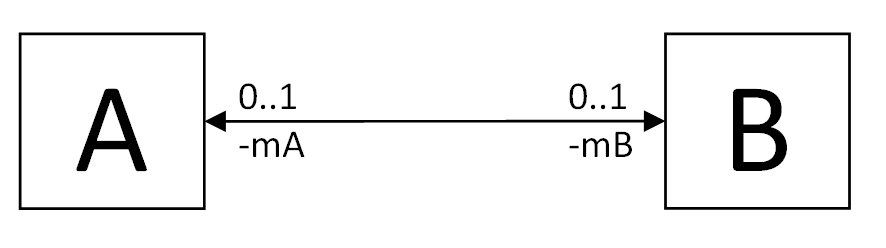
\includegraphics[width=5cm]{./bilder/Assozi_01_01.png}

\textbf{Header B:}
\begin{lstlisting}
class A; // Vorwaertsdeklaration

class B {	
	public:
		B();
		void setA(A* pA);
		A* getA();
		
	private: 
		A* mA; // Pointer auf A-Objekt
};
\end{lstlisting}

\textbf{Aufruf:}
\begin{lstlisting}
A a;
B b;
a.setB(&b);
\end{lstlisting}
\end{multicols}

\subsubsection{"`1:0..1"'}
Eine 1:0..1 Assoziation kann ähnlich wie eine 0..1:0..1 Assoziation
implementiert weden. Wobei auf der "`1 Seite"' die andere Klasse direkt im
Konstruktor mitgegeben wird. Ein Setter wird auf der B-Seite nicht mehr
gebraucht! Achtung: untenstehende Implementation zeigt nur schematisch auf wie
es funktioniert. Copy- und Zuweisungskonstruktor müssten auch noch korrekt
implementiert werden.
\begin{multicols}{2}
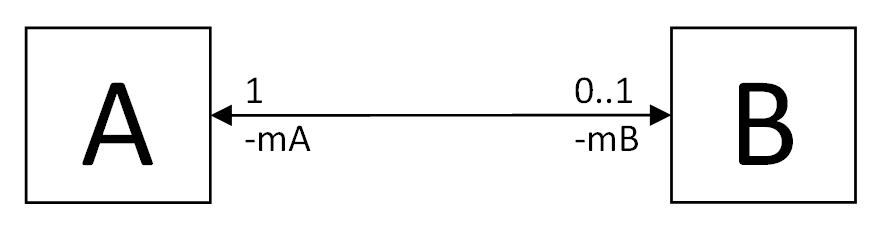
\includegraphics[width=5cm]{./bilder/Assozi_1_01.png}\\
\textbf{Header B (Muss Assoziation)}
\begin{lstlisting}
// ...
class B {
	public: 
		A* getA();
		B(A* pa);		// Konstruktor
	
	private:
		A* mA;		
		B();			// Default Konstruktor
}
\end{lstlisting}
\columnbreak
\textbf{Implementation B (Muss Assoziation)}
\begin{lstlisting}
B::B(A* pA)
: mA(pA)
{
	mA->setB(this); 
	// Kann auch im im Aufruf erfolgen
}
\end{lstlisting}

\textbf{Aufruf:}
\begin{lstlisting}
	A a;
	B b(&a);
\end{lstlisting}
\end{multicols}

\newpage

\subsubsection{"`0..1:0..n"'}
\begin{multicols}{2}
\textbf{Header A:}
\begin{lstlisting}
class B; // Vorwaertsdeklaration

class A{
	private:
		B* mB[n]; // Pointerarray auf B-Objekte
	
	public:
	    A();
		void addB(B* pB);
		void removeB(B* pB);
};
\end{lstlisting}

\textbf{Implementation:}
\begin{lstlisting}
A::A() {
	for(int i = 0; i<n; i++) {
		// Alle Werte auf 0 initialisieren
		mB[i] = 0; 
	}
}

// fuer removeB sinngemaess (->setA(0); mB[i]=0)
void A::addB(B* pB) {
	for(int i = 0; i<n; i++) {
		if(mB[i] == 0) {
			mB[i] = pB;
			mB[i]->setA(this);
			return;
		}
	}
}
\end{lstlisting}

\columnbreak
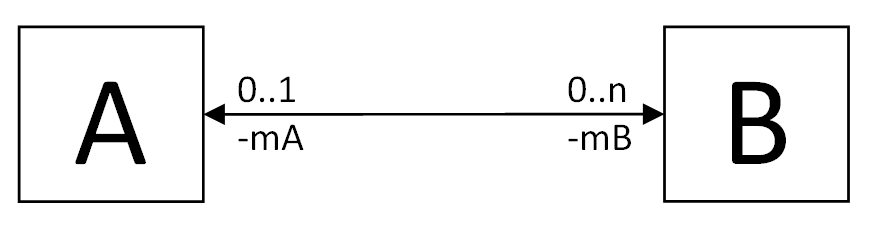
\includegraphics[width=5cm]{./bilder/Assozi_01_0n.png}\\
\textbf{Header B:}
\begin{lstlisting}
class A; // Vorwaertsdeklaration

class B {
	private: 
		A* mA; // Pointer auf A-Objekt
		
	public:
		B();
		void setA(A* pA);
		A* getA();
};
\end{lstlisting}

\textbf{Aufruf:}
\begin{lstlisting}
A a;
B b1;
B b2;
a.addB(&b1);
a.addB(&b2);
a.removeB(&b2);
// ...
\end{lstlisting}
\end{multicols}

\subsection{Vererbung}
\begin{multicols}{2}
\textbf{Basisklasse}
\begin{lstlisting}
	class: Fahrzeug
	{
	public:
			 Fahrzeug(int pGewicht);
		void setGewicht(int pGewicht);
	
	private:
		int mGewicht;
	};
\end{lstlisting}

\columnbreak

\textbf{abgeleitete Klasse}
\begin{lstlisting}
	class: Auto : public Fahrzeug
	{
	public:
			 Auto(int pPersonen, int pGewicht);	
		void setPersonen(int pPersonen);
		
	private:
		int	mPersonen;
	}	
\end{lstlisting}
\end{multicols}

\textbf{Aufruf}
\begin{lstlisting}
	Auto.setGewicht(42);
	Auto.setPersonen(4);
\end{lstlisting}




